\documentclass[fleqn, 14pt]{extarticlej}
\oddsidemargin=-1cm
\usepackage[dvipdfm]{graphicx}
\textwidth=18cm
\textheight=23cm
\topmargin=0cm
\headheight=1cm
\headsep=0cm
\footskip=1cm

\def\labelenumi{(\theenumi)}
\def\theenumii{\Alph{enumii}}
\def\theenumiii{(\alph{enumiii})}
\usepackage{comment}
\usepackage{indentfirst}
\begin{document}
%%%%%%%%%%%%%%%%%%%%%%%%%%%%
%% 表題
%%%%%%%%%%%%%%%%%%%%%%%%%%%%
\begin{center}
{\Large {\bf EnCalの改善案}}

\end{center}
\begin{flushright}
2013年5月30日

乃村研究室 河野 達生
\end{flushright}


\section{はじめに}
自身の研究が情報の可視化,整理に決定した.カレンダの情報を扱うことを想定しているため,実際にEnCalを使用した.EnCalについては次章で説明する.本資料は,EnCalを使用し,改善案を考察したものである.

\section{EnCalとは}
EnCalとは,作業発生の規則性を扱うカレンダシステムである\cite{book1}.
現在EnCalの作業発生の予測手法に,過去の手法が用いられている\cite{book2}.
図1にEnCalのUIを示す.EnCalのUIは以下の4つから構成されている.

\begin{enumerate}
	\item 主として操作するカレンダ\\
	主として操作するカレンダは,タスクを登録できる.また,MissionsやEvent Forecastingからドラッグアンドドロップすることでタスクを登録できる.
	\item 過去のカレンダ\\
	過去のカレンダは,主として操作するカレンダと同様の機能を持つ.過去のカレンダに登録されているタスクを主として操作するカレンダにドラッグアンドドロップすることで,タスクを登録できる.
	\item Missions\\
	Missionsは,関連性をもつタスクをまとめたMissionsの一覧.
	\item Event Forecasting\\
	Event Forecastingは,予測されたタスクの一覧.

\end{enumerate}

\begin{figure}[h]
  \begin{center}
    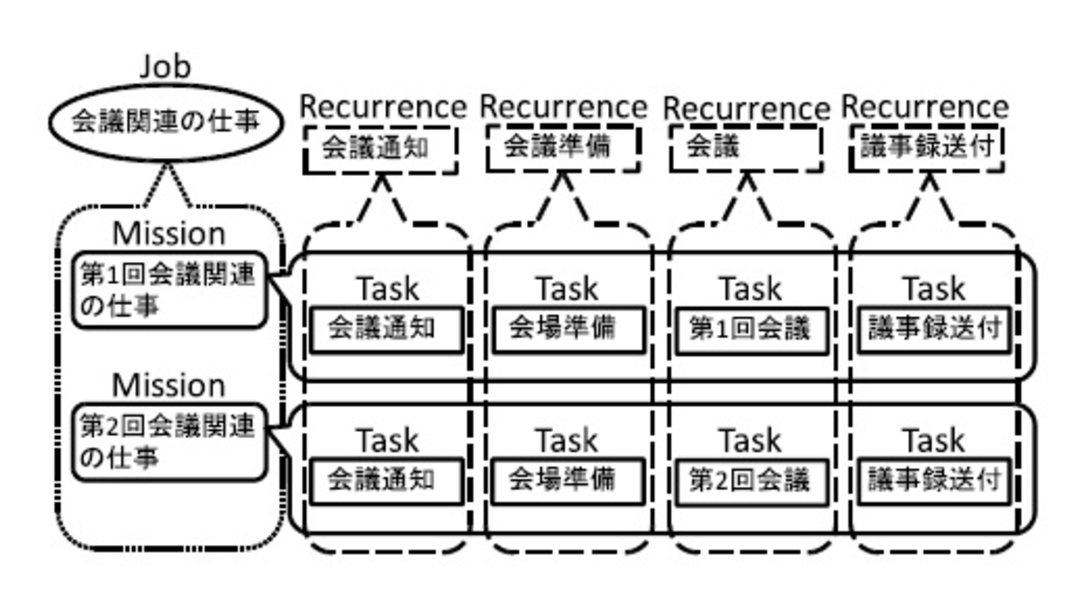
\includegraphics[clip,width=1\columnwidth]{zu3.eps}
    \caption{EnCalのUI}
  \end{center}
\end{figure}

\newpage
\section{改善案}
既存のUIに対する問題点と,これに対する改善案を考察した.考察した5つの問題点と改善案を以下に述べる.

\begin{enumerate}
	\item MissionsとEvent Forecastingは,スクロールに従い追随し視界から消えないようにする.\\
月の下旬を参考にするために画面を下にスクロールすると,MissionsとEvent Forecastingが見えなくなってしまう問題がある.
これにより,MissionsとEvent Forecastingの一覧からドラッグアンドドロップでの登録が困難になる.
MissionsとEvent Forecastingは,使用頻度が高いと思われるため,スクロールに追随するように改善する.\\
	
% 	\item MissionsとEventForecastingのタスクは,.\\
% 	(理由) 予想されるタスクを表示されているが,必ずしも表示されている月に予定が入るとは限らないためである.

% 	\item Missionsから作成された予定を削除する際.Missions単位で削除するかタスク1つを削除するか選択できるようにする.\\
% 	(詳細) Missionsからタスクを作成する際,複数タスクが作成される.しかし,ユーザが誤ってMissionsからタスクを作成した場合,各タスクごとに削除を行わなければならない.そのため,Missions単位で削除するか,タスク1つを削除するか選択できるように改善する.
	
	\item 未来のカレンダを表示する.\\
ユーザは過去のカレンダから主として操作するカレンダにドラッグアンドドロップすることによりタスクを登録できる.
しかし,主として操作するカレンダに登録されているタスクを未来のカレンダに登録する場合,一度過去のカレンダの表示月を変更し,未来のカレンダとしなければならない問題がある.
例えば,今年度から開催される勉強会のタスクを作成する.過去に発生したことがないタスクであるため,過去のカレンダを表示する必要はなくなる.
そこで未来のカレンダを表示させることでユーザの作業を支援するよう改善する.

% 主として操作するカレンダに登録されているタスクを過去のカレンダを表示し,各カレンダの表示月を変更する操作が必要である.
% この操作は手間であるため,過去のカレンダを表示させる機能と同様に,未来のカレンダを表示させる機能を追加することで,使いやすく改善する.
% に登録されているタスクを参照し,計画立案を行うことがある.しかし,過去に発生したことがないタスクを作成する場合,現在のカレンダのタスクから未来のカレンダにタスクを登録する必要がある.この場合,問題がある.

	\item 次回の開催回数を予測する.\\ 
“第○○”という名前のタスクには,周期性があるものが多い.
Event Forecastingからタスクを作成する際,“第○○+1”と名前を変更しなければならない問題がある.
このため,Event Forecastingに予測されている段階で,“第○○+1”と表示されるように改善する.
例えば,”第21回開発打合せ”のタスクを終え,次回のタスクが予測される場合,“第22回開発打合せ”と予測されるよう改善する.
	
	\item 複数の予定を扱えるようにする.\\ 
複数のタスクからMissionsを作成することや一度に複数のタスクを削除することは,頻繁に起こると考えられる.
現在では,各タスクごとにミッションを作成する作業や削除する作業が必要になる.この作業は,ユーザにとって手間だという問題がある.
複数のタスクを扱うために,タスクの横にチェックボックスを作成して,扱えるように改善する.

	\item プロジェクトごとでカレンダを切り替えられるようにする.\\ 
ユーザのロールによって使用するカレンダが,異なる可能性がある.ロールをプロジェクトと表し,プロジェクトごとに分けられるように改善する.

\end{enumerate}

\section{考察}
3章に改善案を記載した.しかし,EnCalのコードをまだ理解していないため,私の主観に依存している部分が多いと考えられる.コードの理解に加え,周囲の意見を参考に実装する必要があるか検討しなければならない.

\begin{thebibliography}{99}
  \bibitem {book1}
三原俊介,谷口秀夫,乃村能成,南裕也:作業発生の規則性を扱うカレンダシステムの評価,情報処理学会論文誌,Vol.540,No.2,pp.630-638(2013).
  \bibitem {book2} 
吉井英人,乃村能成,谷口秀夫:作業発生の規則性に基づく作業予測手法,マルチメディア通信と分散処理ワークショップ論文集, vol.2012, no.4, pp.58-64 (2012).

\end{thebibliography}

\end{document}
